\documentclass[12pt, twoside]{article}
\usepackage[francais]{babel}
\usepackage[T1]{fontenc}
\usepackage[latin1]{inputenc}
\usepackage[left=6mm, right=6mm, top=6mm, bottom=3mm]{geometry}
\usepackage{float}
\usepackage{graphicx}
\usepackage{array}
\usepackage{multirow}
\usepackage{amsmath,amssymb,mathrsfs}
\usepackage{soul}
\usepackage{textcomp}
\usepackage{eurosym}
 \usepackage{variations}
\usepackage{tabvar}


\pagestyle{empty}

\begin{document}


\section*{\center{Devoir maison 3}}

\textit{Devoir � rendre sur feuille grand format petits
carreaux pour le \ul{vendredi 18 d�cembre 2009}.}

\enskip


\textit{Remarque: La r�daction et la justifcation des r�sultats seront pris en
compte (et ont autant d'importance que les calculs).}

\subsection*{Exercice 1}

\begin{enumerate}
  \item VAR est un triangle rectangle en A tel que VA=15cm et VR=17cm. Calculer
  la longueur AR.
  \item POT est un triangle rectangle en O tel que PO=120m et TO=119m. Calculer
  la longueur TP.
\end{enumerate}



\textit{Indications: Commencer par faire un sch�ma.} 


\textit{On rappelle que mesurer sur la figure n'est pas une preuve.}



\subsection*{Exercice 2}

Les triangles suivants sont-ils rectangles? Justifier votre r�ponse.

\begin{center}
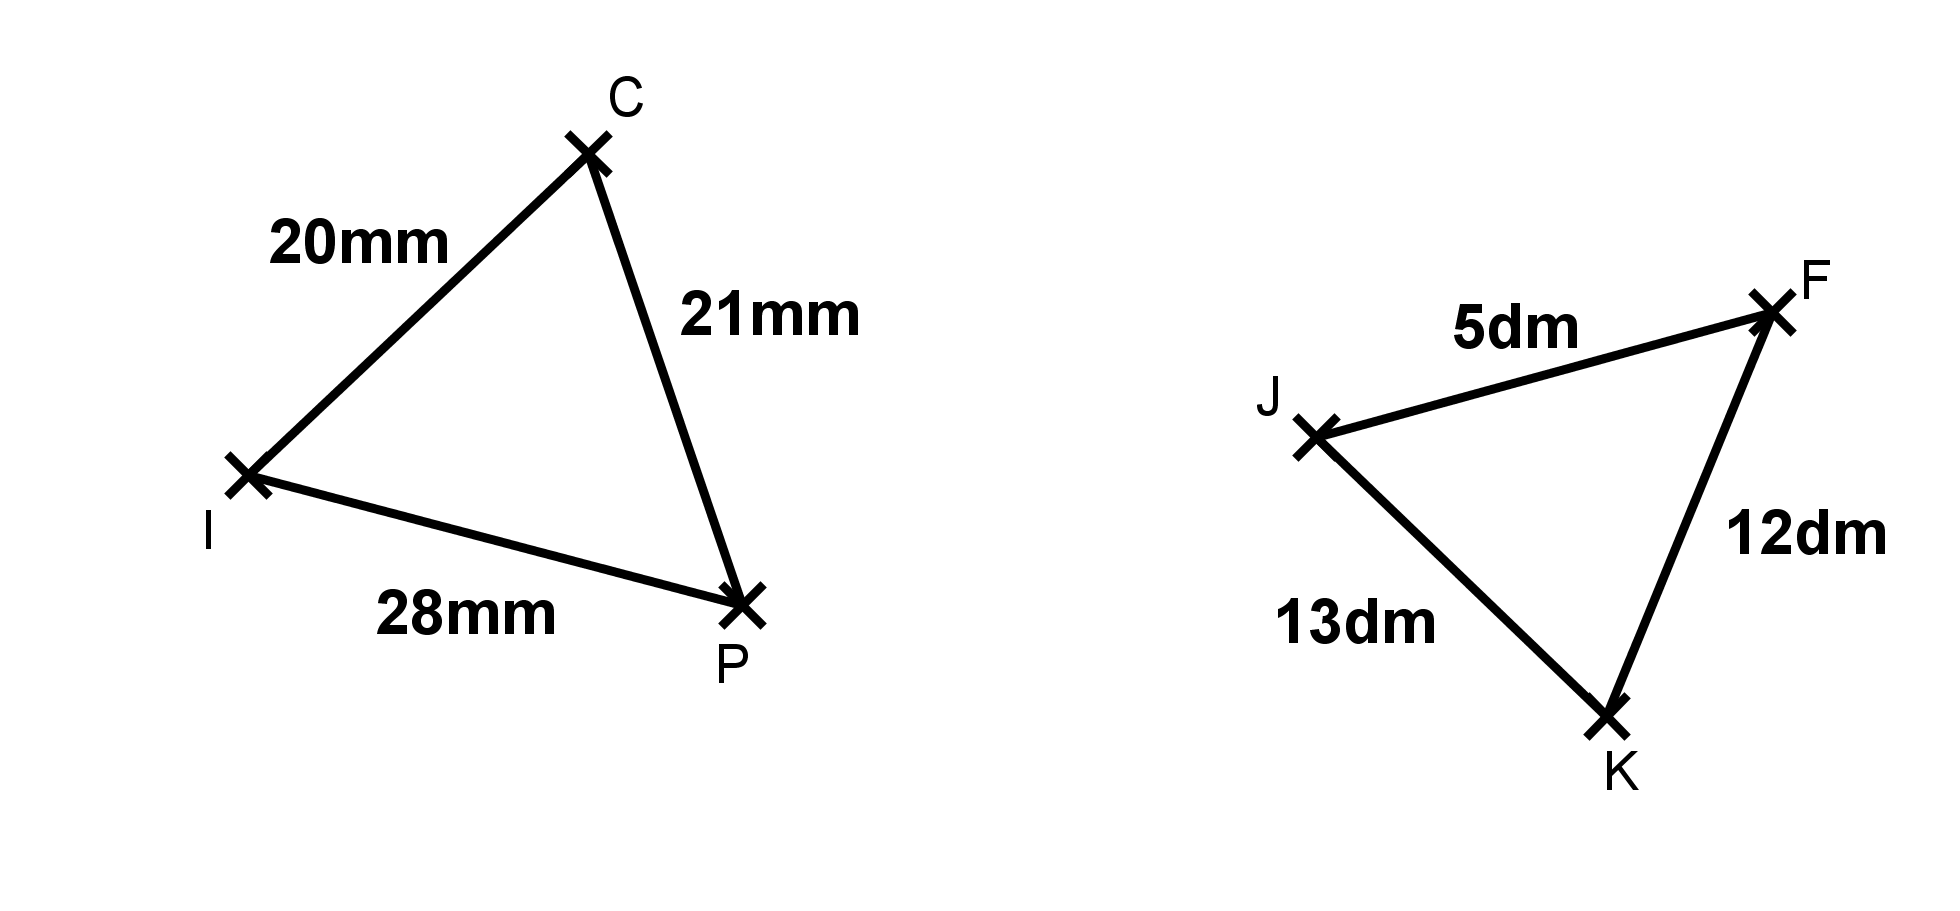
\includegraphics[width=10cm]{images/tri1.png} 
\end{center}






\subsection*{Exercice 3}


Elodie encadre un tableau (rectangulaire). Pour cela, elle veut d�couper un
morceau de verre rectangulaire. Le morceau d�coup� mesure 36cm et 48cm de c�t�
et 59cm de diagonale. Elodie a-t-elle bien r�ussi sa d�coupe? (commencer par faire un sch�ma du morceau
de verre.)


\subsection*{Exercice 4}

A partir des informations de la figure:

\begin{center}
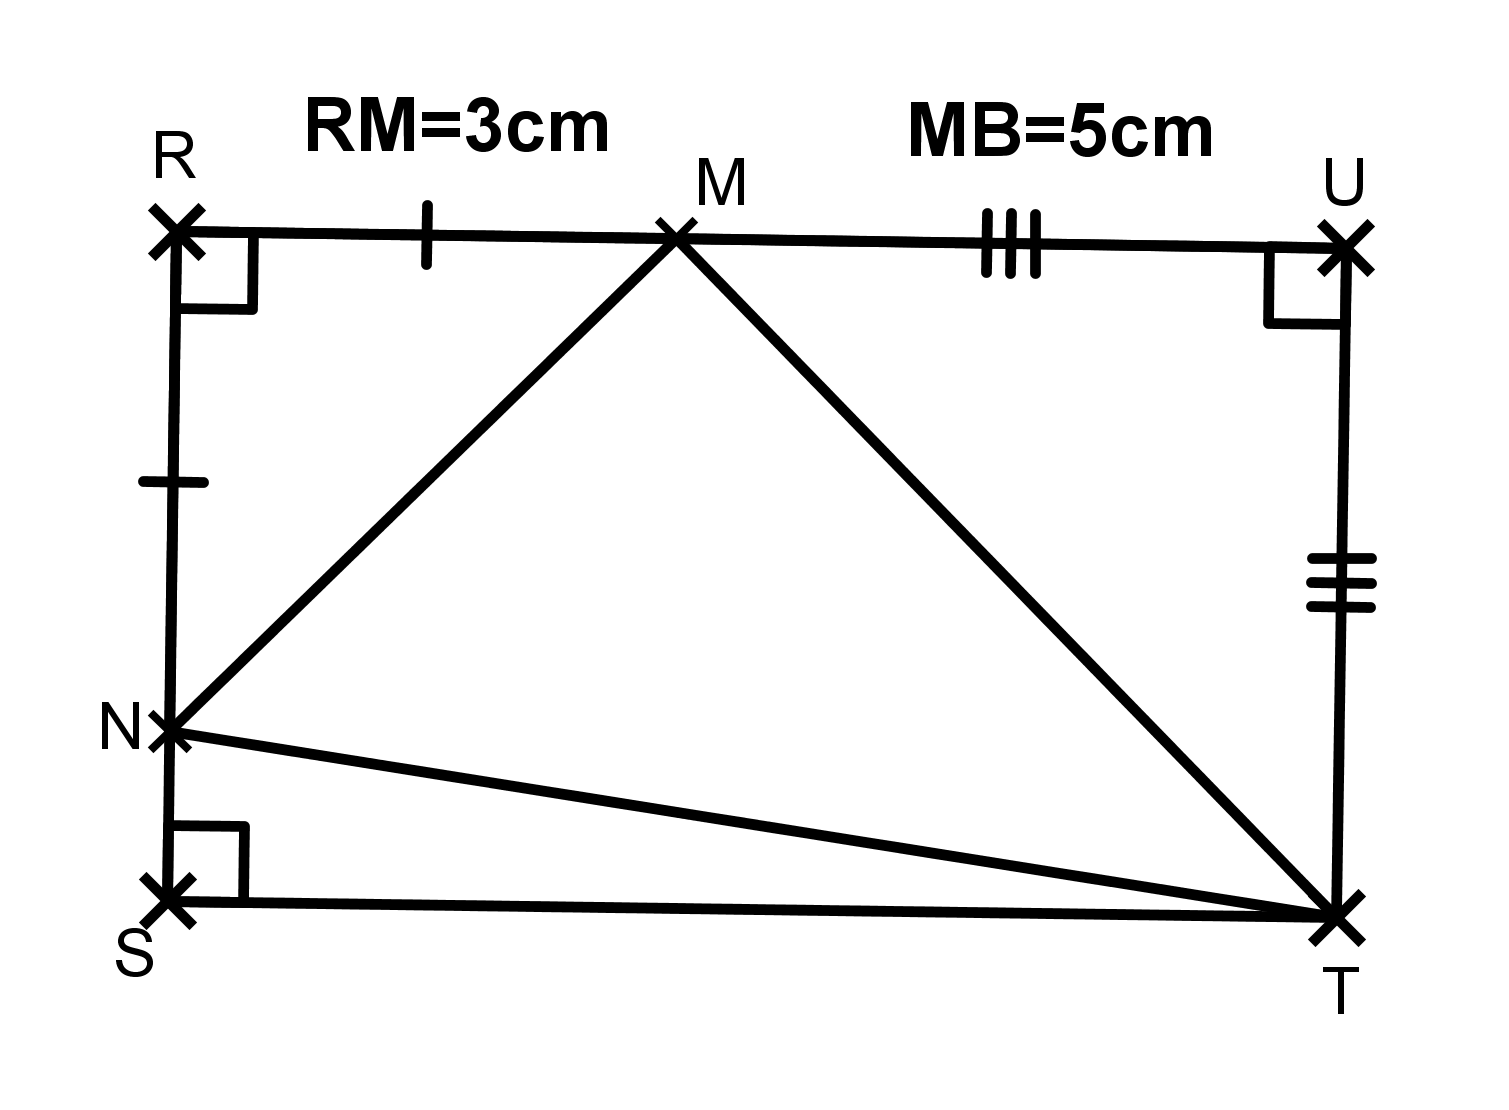
\includegraphics[width=7cm]{images/ex4.png}
\end{center}

\begin{enumerate}
  \item Calculer MN, MT et NT. 
  \item Le triangle MNT est-il un triangle rectangle? Justifier votre r�ponse.
  (Indication: Garder les valeurs exactes de la question pr�c�dente.)
 
\end{enumerate}
\pagebreak


\section*{\center{Devoir maison 3}}

\textit{Devoir � rendre sur feuille grand format petits
carreaux pour le \ul{jeudi 17 d�cembre 2009}.}

\enskip


\textit{Remarque: La r�daction et la justifcation des r�sultats seront pris en
compte (et ont autant d'importance que les calculs).}


\subsection*{Exercice 1}

\begin{enumerate}
  \item VAR est un triangle rectangle en A tel que VA=15cm et VR=17cm. Calculer
  la longueur AR.
  \item POT est un triangle rectangle en O tel que PO=120m et TO=119m. Calculer
  la longueur TP.
\end{enumerate}



\textit{Indications: Commencer par faire un sch�ma.} 


\textit{On rappelle que mesurer sur la figure n'est pas une preuve.}



\subsection*{Exercice 2}

Les triangles suivants sont-ils rectangles? Justifier votre r�ponse.

\begin{center}
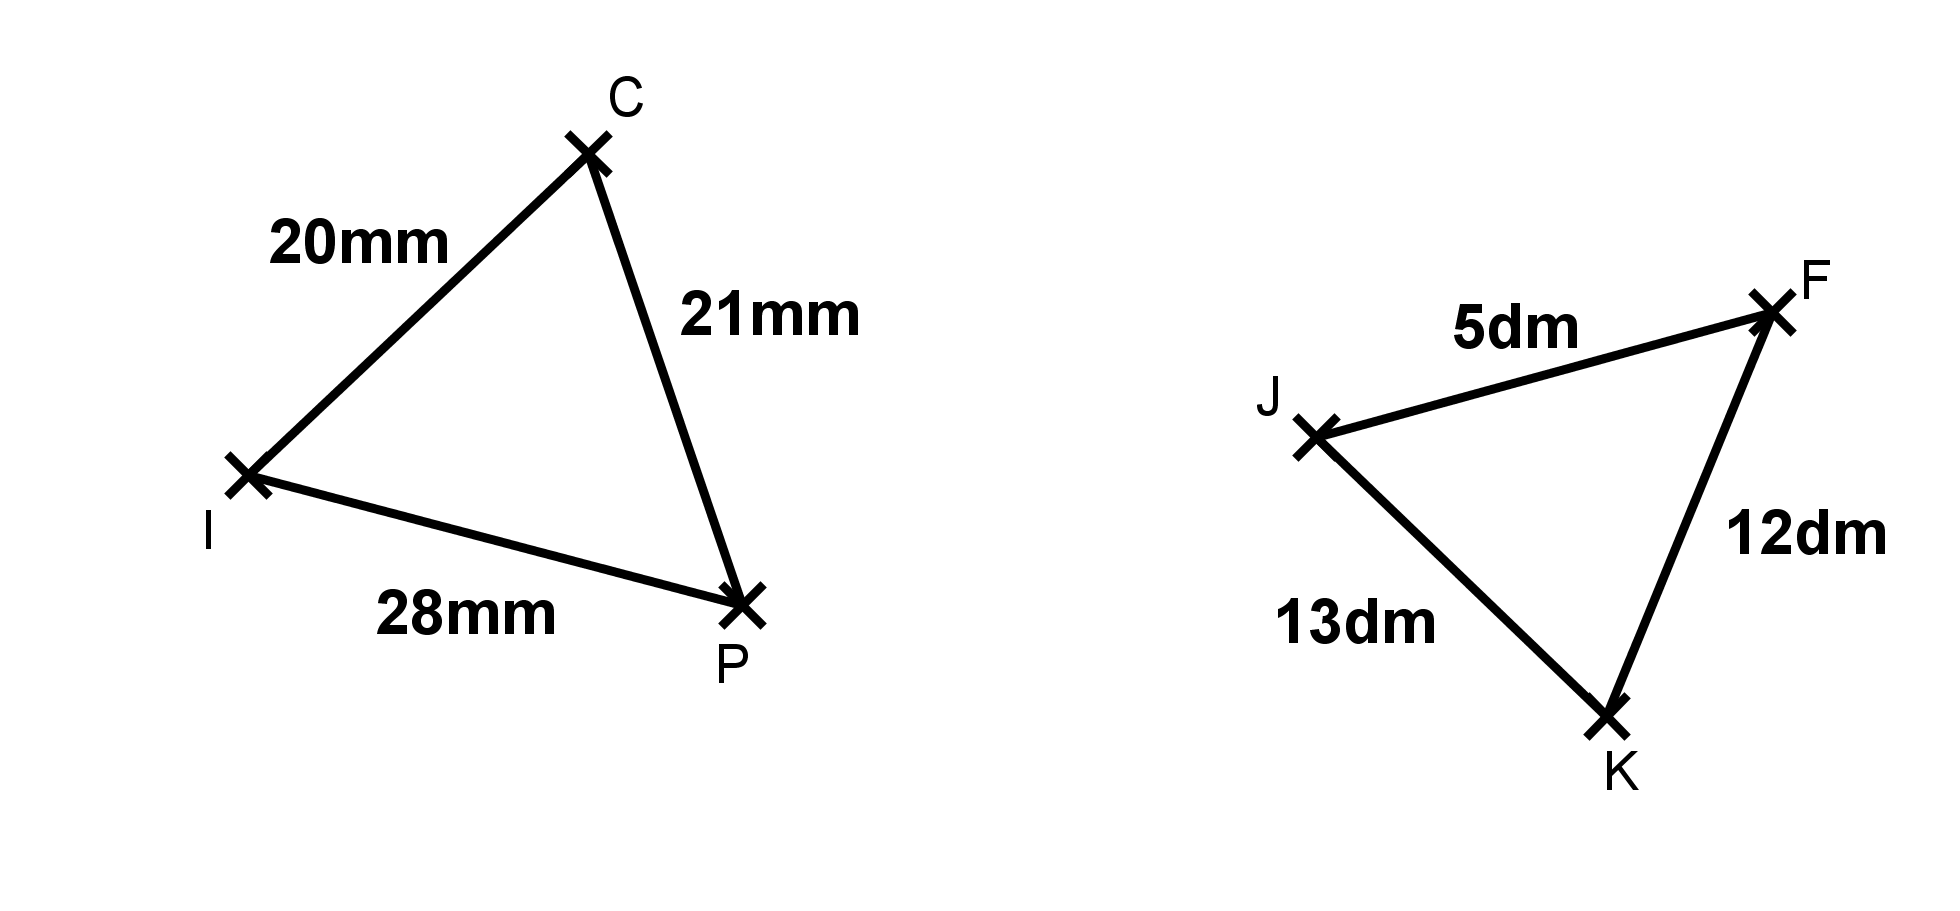
\includegraphics[width=10cm]{images/tri1.png} 
\end{center}



\subsection*{Exercice 3}

\begin{enumerate}
  \item Tracer un segment [AB] de longueur 7cm.
  \item Tracer le cercle de diam�tre [AB] puis placer sur ce cercle le point C
  tel que BC=4,5cm.
  \item Que peut-on dire du triangle ABC? Justifier votre r�ponse.
  \item Calculer la longueur AC au millim�tre pr�s.
\end{enumerate}

\subsection*{Exercice 4}

Un arbre s'est bris� en deux en tombant sur un mur de 2,5m de haut. Le pied de
l'arbre est situ� � 4m du pied du mur et la cime de l'arbre s'est retrouv� � 6m
du mur.

On cherche la hauteur totale de l'arbre.

\begin{enumerate}
  \item Faire un sch�ma � main lev�e en nommant les diff�rents points (de votre
  choix) et en reportant les donn�es de l'�nonc�.
  \item Calculer la hauteur de l'arbre 
  
\end{enumerate}

 \textit{Indications: on pourra commencer par calculer les longueurs
 manquantes.}

\end{document}
